This section will focus on the tools and techniques used to create a web application tShreyashVardhan2024o manage time and space resources of an organization.


\section{Defining the toolbelt}\label{sec:defining-the-toolbelt}
% Расписать все варианты и в итоге выбрать итоговый.
% Расписать всю структуру будущюю.
% Интересные инструменты использованные указать.

% Spring Boot vs. Spring vs. C# vs. Django vs. Flask
For the programming language, the options were as follows: Java Spring Boot framework, C\#.NET, and Python's Django and Flask.
C\# was first removed, as learning about it would take a considerable amount of time.
Python's Flask is easy to use, but not customizable enough.
Subsequent analysis, as presented in the study~\cite{ShreyashVardhan2024}, indicates that Spring Boot exhibits superior performance.
Moreover, my familiarity with Java might reduce the time required for development.
Consequently, Spring Boot is selected as the back-end framework.
Spring Boot, which is constructed on the Spring Framework, is recognized as a leading framework within the Java ecosystem due to its widespread popularity.
It streamlines the original Spring Framework, thereby facilitating more straightforward maintenance and expediting deployment procedures.
Henceforth, to maintain clarity, the term Spring Boot shall be used exclusively in reference to both the Spring Framework and Spring Boot.

% Google Web Toolkit vs. Thymeleaf vs. React/other JS
An often-utilized integration of back-end and front-end frameworks with Spring Boot is accomplished through Thymeleaf, a template rendering engine which processes page rendering on the server side, thereby reducing computational demand on the client-side systems.
However, alternative solutions are available, including the currently prevalent React framework along with other JavaScript frameworks.
Opting for these alternatives requires considerable investment in research.
Given my proficiency in HTML, the Thymeleaf template system presents a straightforward learning curve.
Nevertheless, a certain degree of JavaScript is essential for contemporary websites, thereby necessitating its use for handling specific tasks such as requests.


% PostgreSQL vs. NoSQL vs. others
For our database, PostgreSQL was chosen, as it is a popular ACID-compliant database.
ACID stands for:
\begin{itemize}
    \item \textbf{Atomicity}: Transaction is either fully completed, or not, with no in-betweens.
    \item \textbf{Consistency}: Guarantees that a transaction brings the database from a valid state to a valid state.
    \item \textbf{Isolation}: Concurrent transactions do not interfere with each other.
    \item \textbf{Durability}: Once a transaction is committed, it stays committed.
\end{itemize}

\section{Introduction to Spring Boot}\label{sec:introduction-to-spring-boot}

Spring Boot is a tool that allows the programmer to create a web server that uses the Model-View-Controller pattern, MVC for short.

The model is a part responsible for the data logic.
The connection to the database, the processing of the requested data and other back-end transactions are what this part consists of.

The view is a part that displays the data to a user or gathers them from them.
Whether HTML, plain text, or any other format such as our Thymeleaf.

The controller is a connector between the previous two, where the data is additionally processed before being sent into either the database or a client of a user.


\section{Schema of the database}\label{sec:schema-of-the-database}
\begin{figure}[h]
  \centering
  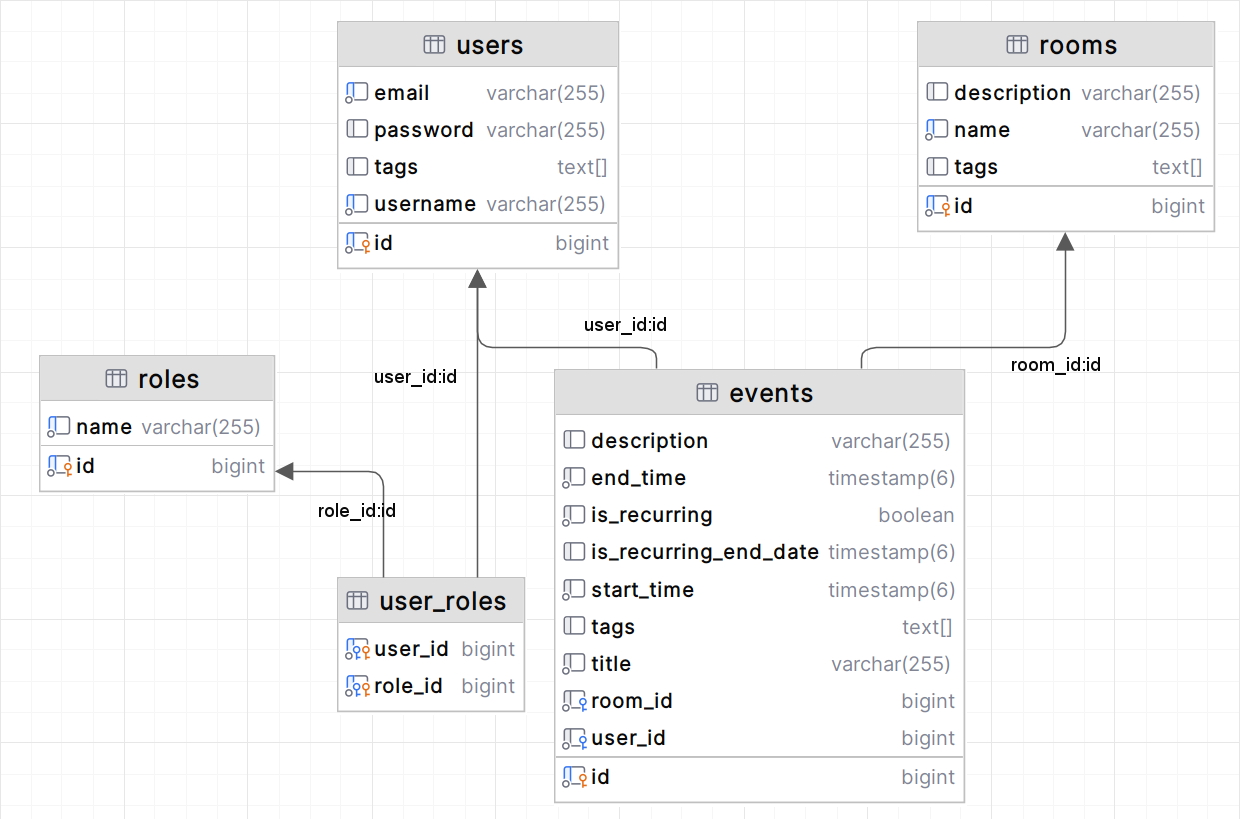
\includegraphics[width=0.6\textwidth]{schemaDB}
  \caption{Schema of the database for the application}
  \label{fig:schemaDB}
\end{figure}

\subsection*{Database \ref{fig:schemaDB} Architecture}

\begin{itemize}
  \item \textbf{users}: Stores user credentials and personal data.
  Each user has a unique \texttt{ID}.

  \item \textbf{roles} \& \textbf{user\_roles}: Implements role-based access control via a many-to-many relation between users and roles.

  \item \textbf{rooms}: Contains information on event locations.
  Each room has a \texttt{name}, \texttt{description} and a unique \texttt{ID}.

  \item \textbf{events}: Represents scheduled activities.
  Includes data such as  \texttt{is\_recurring}, \texttt{title}, \texttt{start\_time} and \texttt{end\_time}.
  Each event references a \texttt{user} and a \texttt{room} that were assigned to this event.

  \item \textbf{users, events }and \textbf{rooms} all contain \texttt{tags} to help categorize them.
\end{itemize}


\newpage%                    NEW PAGE HERE !!!!!!!!!!!!!!!!!!!!!!!!!!!!!!!!!!!!!!!!!!!

\section{The implementation of a Spring Boot application}\label{sec:the-implementation-of-a-spring-boot-application}
In our application, the main controller is CalendarController.
It renders the main page /calendar.
The non-required parameters of a request are: ``\textit{date}'', ``\textit{roomIds}'' and ``\textit{userIds}''.

Parameter \("\)\textit{date}\("\) is simply the day of the week the calendar renders.
If not provided, we use the default value of a current day.

Parameters ``\textit{roomIds}'' and ``\textit{userIds}'' are used to filter out which events the user wants to see in their calendar.
If not provided, events from every room and every user are displayed.

In this controller a week around the current day is generated, all the events that are happening in that week are found and are put into an array that is then sent with the model.


\subsection{Useful tools}\label{subsec:useful-tools}
In this application, \textit{Lombok} was used to reduce the amount of boilerplate code.
It allows for the usage of annotations such as \texttt{@Getter,@Setter} to automatically generate setters and setters for all fields that need them.
In addition, annotations \texttt{@AllArgsConstructor,@NoArgsConstructor} can automatically create the correct construction function for the class.
Finally, \texttt{@Data} combines \texttt{@Getter,@Setter} and some more functions in one annotation, so the classes remain clean and functional.

The use of the tool is demonstrated in the list~\ref{lst:room-class}.
It can be seen that no setter or getter functions are needed, no construction function is needed, and the class looks clean and complete.


\begin{listing}[H]
\begin{minted}{java}
@Data
@Entity
@Table(name = "rooms")
public class Room {
    @Id
    @GeneratedValue(strategy = GenerationType.IDENTITY)
    private Long id;

    @Column(nullable = false, unique = true)
    private String name;

    @Column()
    private String description;

    @Type(io.hypersistence.utils.hibernate.type.array.ListArrayType.class)
    @Column(name = "tags", columnDefinition = "text[]")
    private Set<String> tags = new HashSet<>();
}
\end{minted}
\caption{Lombok-annotated JPA entity}
\label{lst:room-class}
\end{listing}


\newpage%                    NEW PAGE HERE !!!!!!!!!!!!!!!!!!!!!!!!!!!!!!!!!!!!!!!!!!!

\subsection{The architecture of the application}\label{subsec:the-architecture-of-the-application}

The main file responsible for most tasks is CalendarController, where the \texttt{/calendar} endpoint is located.

The \texttt{/calendar} takes 3 non-required parameters.
\begin{itemize}
    \item \textbf{date}: Show the events that happen on the week of the day sent.
    \item \textbf{userIds}: Filter the users shown on the central calendar.
    \item \textbf{roomIds}: Filter rooms displayed in the central calendar.
\end{itemize}

The \texttt{/calendar} then sends these data to \texttt{calendar.html}:
\begin{itemize}
    \item \textbf{userIds} \& \textbf{roomIds} (if supplied from request).
    \item \textbf{selectedDate} (if not provided, current date is used).
    \item \textbf{nextWeek} \& \textbf{previousWeek} to enable navigation within weeks.
    \item \textbf{currentWeekStart}.
    \item \textbf{weekDays} - a list of events that take place on a specific day.
    \item \textbf{eventRepository}, \textbf{userRepository} and \textbf{roomRepository}
\end{itemize}


%Continue describing all endpoints???